\section{Introduction}
Given that stars make up the fundamental blocks of the Galaxy, stellar clusters (SCs) therefore act as important astrophysical laboratories ideal for understanding the Galaxy's dynamics and structure. Stars are well known to be born in cohorts within molecular clouds, dissolving into the interstellar medium to form the field stars that can be seen today. From current star formation theory we know that the youngest of these clusters where formed from a singular burst of star formation, and are therefore referred to as \textit{simple stellar populations} (SSPs), groups of chemically homogeneous stars \autocite{huangDrivingFactorsMultiple2024}. These groups are known as \textit{open clusters} (OCs) due to their loosely-bound and irregular appearance. OCs also tend to exhibit lower total stellar masses, and are primarily located in the Galactic disk \autocite{zwartYoungMassiveStar2010a}. OCs can be used as tracers for studying galactic spiral structure \autocite{dias58OpenClusters2022}.

Globular clusters (GCs), on the other hand, are high-density collections of stars, distributed throughout the Galactic halo. GCs are found to be in a more stable virial state, with an older age distribution as well as higher dynamical timescales, which contributes to their spherically symmetrical appearance. As a result of their larger age, GC populations tend to be more complex, to the point that they sometimes cannot be properly described as a SSP; chemical abundance variations between stars in a single GC indicates \textit{multiple stellar populations} (MPs) with later-generation stars showing distinct chemical compositions \autocite{huangDrivingFactorsMultiple2024}. Although they have historically been studied as a separate category from OCs, current models do not discriminate between either OCs or GCs for describing their dynamics and compositions \autocite{krumholzStarClustersCosmic2019}.

The characterization of SCs typically involves two processes: the identification of member stars and their separation from the surrounding field stars, and the determination of the SC's fundamental parameters. Of particular relevance to this project is the study of SCs through theoretical isochrone fitting procedures using multiband observations.

\subsection{Membership Determination}

Many different approaches to discriminate SCs from a population of field stars have been proposed and employed in the literature with varying degrees of success. While early methodologies generally relied on spatial coherence, later surveys and multi-epoch photometric observations allowed for the consideration of kinematic coherence between cluster stars, eventually giving way to the clustering techniques used in more recent works on stars' astrometric solutions \autocite{ramezaniDifferentMethodsCalculate2026}. While this project utilizes HDBSCAN as discussed in Section \ref{sec:membership}, other statistical approaches include a forest fire inspired model \autocite{weiForestFireClustering2025}, Gaussian mixture models, K-means, etc. \autocite{peraPyUPMASKImprovedUnsupervised2021}.

The Gaia mission \autocite{gaiacollaborationGaiaMission2016b} brought about a revolution in the study of Galactic SCs. Its unparalleled astrometric precision of over 1 billion sources in Data Release 1, and over 2 billion sources in the upcoming Data Release 4, allows for cluster identification at unprecedented scales. Systematic searches have revealed hundreds of previously unidentified clusters throughout the Galaxy \autocite{castro-ginardHuntingOpenClusters2022,huntImprovingOpenCluster2021}. Additionally, Gaia data has been extensively used to refine cluster membership lists \autocite{perrenUnifiedClusterCatalogue2023,huntImprovingOpenCluster2024a}, allowing for studies on clusters' structure \autocite{mendesBATEIA1ApproachDetermining2026,tarricqStructuralParameters3892022a}.

% TODO: maybe mention Grondin extra-tidal stars

\subsection{Cluster Characterization}

Photometric studies of SCs involve fitting synthetic isochrones to color--magnitude diagrams (CMDs), and are a common approach to determining a cluster's fundamental parameters \autocite{diasUpdatedParameters17432021}. While spectroscopic data provides a much stronger constraint on stellar chemical abundances \autocite{kosGALAHSurveyImproving2025}, it is rare to have a significant portion of a cluster's member stars with a reliable measurement of their spectral energy distribution, and as such studies are restricted to use spectro-photometric measurements (in spite of this, narrow-band observations can help, for example, in measuring the blanketing of metallic lines \autocite{paunzenCalibrationGaiaDR32026}). Theoretical isochrone morphology depends on the given age and metallicity, while the cluster's distance and total reddening from interstellar extinction displaces the isochrone's sequence. While traditional isochrone fitting methods seek to minimize a likelihood function such as the distance of each star to the nearest isochrone point \autocite{monteiroFittingIsochronesOpen2010}, models such as the \textit{Mixture Model for Open Clusters} (MiMO; \cite{liMiMOCatalogPhysical2025}) explicitly account for field star contamination, eliminating the need for member star discrimination.

Forward modeling of a cluster can also be performed using codes such as \textit{ASteCA} (further described in Section \ref{sec:asteca}), which when combined with tooling designed for solving the inverse problem can yield a cluster's fundamental parameters alongside an estimate of the posterior density function. More recent efforts have also been made with the implementation of  machine learning tools on observed CMDs, allowing for quick parameter inference \autocite{huntImprovingOpenCluster2023a,cavalloParameterEstimationOpen2023,cantat-gaudinPaintingPortraitGalactic2020a}.

\section{Objectives}
Although a variety of studies have been done using CMDs from other catalogs, few studies include observations in near-ultraviolet filters due to the demanding photometric conditions (as a result of atmospheric sensitivity) required to obtain reliable measurements for a cluster's metallicity and age. For this project, we will exploit over 20 years of UBVRI observations of over 1700 resolved Galactic clusters (both GCs and OCs), which can be used to provide reliable measurements of the clusters' fundamental parameters with stronger model constraints than is otherwise possible without UBV observations \autocite{kavirajBetterAgeEstimation2007}. The observations from the \textit{Observatorio Astron\'omico Nacional -- San Pedro M\'artir} (hereafter referred to as SPM) are complemented with photometry obtained from all-sky surveys when available, crossmatching the Gaia observations with GALEX, 2MASS, PAN-STARRS, SDSS, and WISE.

The project's key objectives are outlined as follows:

\begin{itemize}
    \item Determine and expand on stellar cluster membership catalogs using high quality astrometric data, focusing on retrieving faint member stars that were otherwise discarded in previous studies.
    \item Implement existing tools for determining clusters' physical parameters based on cleaned CMDs using revised membership lists.
    \item Develop new tools for the efficient and accurate characterization of cluster CMDs.
    \item Use newly developed tools for determining fundamental and structural parameters of SCs and SC candidates using observations from SPM, supplemented with observations from external catalogs: 2MASS, WISE, GALEX, Gaia, PAN-STARRS, and SDSS when available.
\end{itemize}

\section{Catalog of Observations}
For this project we have observations of over 1700 clusters, compiling the results from 298 observation campaigns dating back to the year 2001. Each observational campaign focuses either on the suspected cluster members, or the foreground or background stars. Doing a preliminary cross-match with the \textit{Unified Cluster Catalog} (UCC; \cite{perrenUnifiedClusterCatalogue2023}) shows over 300 clusters not identified in the UCC, with some having been identified as asterisms (physically unrelated groups of observed stars). As part of the initial data exploration step of the methodology, a more in-depth review of the published literature will be needed to determine the characterization already performed for each cluster in the sample. 

As can be seen in Figure \ref{fig:mw-distribution}, our observations encompass a dense sample the Solar neighborhood, both spatially as well as characterization quality from the UCC UTI metric, providing a good opportunity to improve the worst-scoring clusters and provide a uniform study of the stellar parameter spatial distributions. Thanks to the photometric conditions of at SPM, stars up to a magnitude of $\sim  21$ can be recorded, allowing for a deeper high quality measurement of SC members. This will allow us to obtain quality photometric measurements for a higher amount of low luminosity members, thus reducing selection bias effects as a result of incomplete sampling of low mass members.

\begin{figure}[!ht]
    \centering
    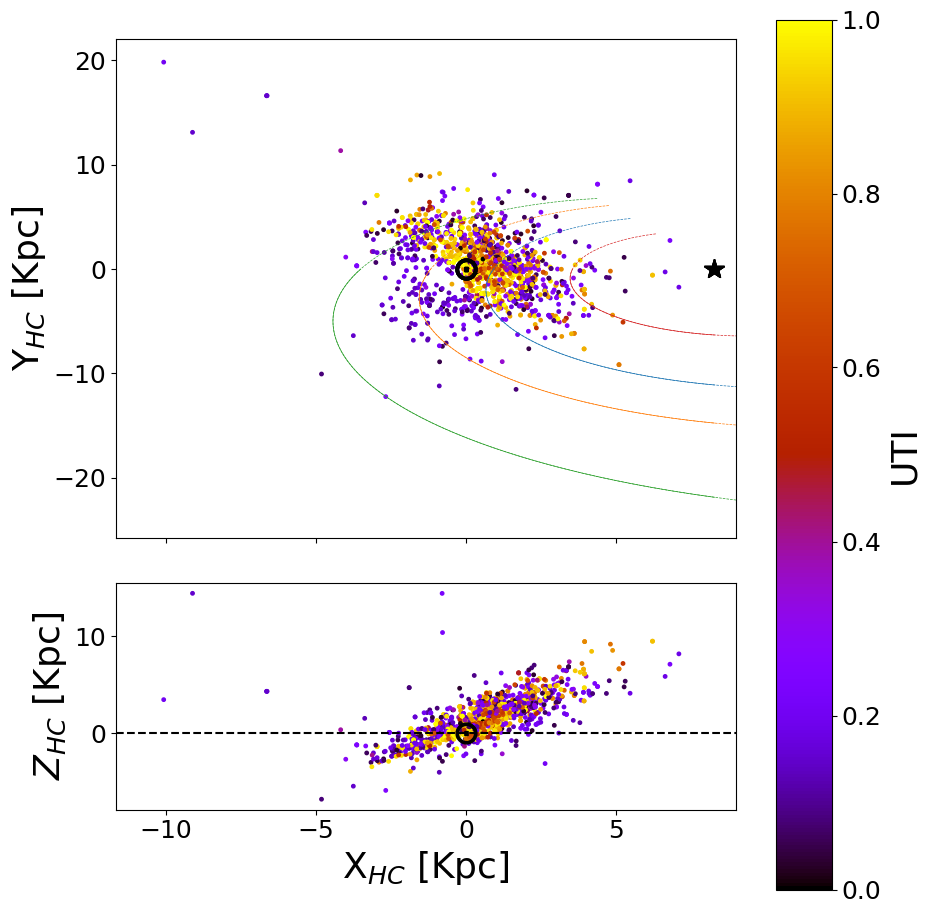
\includegraphics[width=0.85\linewidth]{figures/SPM Milky Way Clusters.png}
    \caption{Spatial distribution of observed SCs in the Galaxy in the Solar neighborhood. Heliocentric coordinates were calculated using distances determined through manual photometric analysis of each cluster.}
    \label{fig:mw-distribution}
\end{figure}

\subsection{Cluster Sample}

As a first test of the membership determination pipeline and preliminary evaluation of the physical characterization of each OC's CMD, we selected four well-studied, well-populated clusters all located within a similar parallax range: \textit{NGC 1245}, \textit{NGC 2311}, \textit{NGC 2420}, and \textit{NGC 2506}. An initial literature distance determination was reported for all but NGC 2311 \autocite{alterCatalogueStarClusters1970}, while subsequent studies have been made in an effort to understand each cluster's fundamental parameters \autocite{liMiMOCatalogPhysical2025,huntImprovingOpenCluster2024a,cavalloParameterEstimationOpen2023} and use them\textemdash as part of a larger sample of Galactic SCs\textemdash to understand and trace the Galactic structure \autocite{cantat-gaudinPaintingPortraitGalactic2020a,kharchenkoGlobalSurveyStar2016}.

Due to the technical limitations of the cluster characterization tooling available at this time we opted to only use each cluster's Gaia DR3 observations, as this would have the most amount of information available and whose broadband passbands cover a portion of the UV spectrum, providing some sensitivity to metallic lines and thus increasing sensitivity to a cluster's global metallicity, albeit without the sensitivity a narrow-band passband might otherwise provide \autocite{paunzenCalibrationGaiaDR32026}.